\chapter{\sffamily Interacting with systems in general}

{\bfseries\sffamily Concept.} To design and build a generalised concept of interacting with stochastic processes of any kind. The mathematical formalism and software that we introduce here will serve as a common language and interface for any simulation studies into manipulating real world phenomena, and should enable the learning of control algorithms. We implement the software as an extension to the stochadex package. For the mathematically-inclined, this chapter will cover how interactions are structured in theory by developing some useful extensions to the stochadex formalism and illustrating with some simple examples. For the programmers, the public Git repository for the code described in this chapter can be found here: \href{https://github.com/umbralcalc/stochadex}{https://github.com/umbralcalc/stochadex}.

\section{\sffamily Formalising general interactions}

\textcolor{red}{Rewrite this section to remove the existence of parametric actions, rewrite the code in the stochadex to match, and make this section more about the kinds of actions that can be performed on the basic stochadex simulations.}

\textcolor{red}{Include a full description of policies here!!}

Let's start by considering how we might adapt the mathematical formalism we have been using so far to be able to take actions which can manipulate the state at each timestep. Using the mathematical notation that we inherited from the stochadex, we may extend the formula for updating the state history matrix $X'\rightarrow X$ to include two layers of possible interactions which are facilitated by a new vector-valued `parametric action' function $G_{{\sf t}}$ and a new vector-valued `state action' function $H_{{\sf t}}$. In doing so we shall be defining the domain of an acting entity in the stochastic process environment --- which we shall hereafter refer to as simply the `agent'.

During a timestep over which actions are performed by the agent, the stochadex state update formula can be extended to look like this system of equations
%%
\begin{align}
Z_{{\sf t}+1}^i &= G_{{\sf t}+1}^i(Z_{{\sf t}}, {\cal A}_{{\sf t}+1}) \label{eq:generalised-param-actions} \\
X_{{\sf t}+1}^i &= H^i_{{\sf t}+1}[F_{\sf t}(X', Z_{{\sf t}+1}, {\sf t}), {\cal A}_{{\sf t}+1}] \label{eq:generalised-state-actions} \,,
\end{align}
%%
where we have also introduced the concept of the `actions' performed ${\cal A}_{{\sf t}+1}$ on the system; some vector of parameters which define what actions are taken at timestep ${\sf t}+1$.

In Eqs.~(\ref{eq:generalised-param-actions}) and~(\ref{eq:generalised-state-actions}), notice that we have replaced the constant vector of parameters $z$ (as in the stochadex formalism) for a time-dependent vector $Z_{{\sf t}}$ of parameters that can be updated by $G_{\sf t}$ at any (but not necessarily every) timestep. From the perspective of the whole matrix $X$ update step; $G_{\sf t}$ and $H_{\sf t}$ combine to become technically equivalent to applying this formal composition of functions
%%
\begin{align}
X^i_{{\sf t}+1} &= H^i_{{\sf t}+1}(F_{\sf t}(X', G_{{\sf t}+1}^i(Z_{{\sf t}}, {\cal A}_{{\sf t}+1}), {\sf t}), {\cal A}_{{\sf t}+1}) = {\cal F}^i_{{\sf t}+1}(X', Z_{{\sf t}}, {\cal A}_{{\sf t}+1}, {\sf t}) \label{eq:action-iteration-formula}\,,
\end{align}
%%
which looks like an absolute mess! However, it illustrates how ${\cal F}$, which refers to a modified version of the $F$ function, contains our actions but no other new parameters need be specified; only function operations. Hence, while we have provided two distinct ways one might encode actions to manipulate a stochastic phenomenon, we shall often just refer to them together as `taking an action' ${\cal A}_{{\sf t}+1}$ at timestep ${\sf t}+1$ --- because the parameters which define either type of action at this timestep should all be stored within ${\cal A}_{{\sf t}+1}$ anyway. It is, however, important not to forget the full mathematical formulation when performing calculations. 

The code for the new iteration formula given by Eq.~(\ref{eq:action-iteration-formula}), which includes taking actions in the same timestep, would look something like Fig.~\ref{fig:iterations-with-actions}.

\begin{figure}[h]
\centering
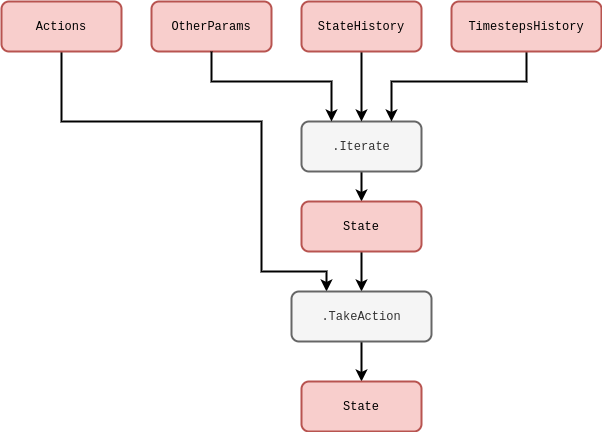
\includegraphics[width=11cm]{images/chapter-9-iterations-with-actions.drawio.png}
\caption{Code schematic of Eq.~(\ref{eq:action-iteration-formula}).}
\label{fig:iterations-with-actions}
\end{figure}

Up to this point, we have only considered actions which were either scheduled up front through some fixed process or through user interaction via a game interface. In order to start creating algorithms to act on the system state for us, we now need to develop a formalism which `closes the loop' by feeding information back from the stochastic process to another decision-making process. Note that in most cases, the state of real-world phenomena cannot be measured perfectly. So in order to enable any agent trained on simulated phenomena to potentially act in the real world, we will need to model this measurement process as part of the information retrieval step.

Let's now define the concept of an `environment state' ${\cal S}_{{\sf t}+1}$ at timestep ${\sf t}+1$; this is a new vector that doesn't have to share the same length as the measured state vector $X_{{\sf t}+1}$. We will then say generally that this environment state is `observed' by the agent using the following observation function
%%
\begin{align}
{\cal S}_{{\sf t}+1}^i &= O_{{\sf t}+1}^i(X',{\cal Z}_{{\sf t}+1},{\sf t}) \label{eq:generalised-state-measurement} \,,
\end{align}
%%
where we have also introduced a new vector ${\cal Z}_{{\sf t}+1}$ which we will use to store all of the relevant parameters to the agent\footnote{This vector is intended to include parameters for measurement, policy specification and ultimately the learning algorithm as well.} at timestep ${\sf t}+1$.

If we are now given the conditional probability that an action vector element ${\cal A}_{{\sf t}+1}=a$ is chosen given that state vector ${\cal S}_{{\sf t}+1}=s$ has been measured $\pi (a,s) = p(a\vert s)$, we can use this to draw new actions for the agent with a newly defined action-generating function
%%
\begin{align}
{\cal A}_{{\sf t}+1}^i &= \Pi_{{\sf t}+1}^i({\cal S}_{{\sf t}+1}, {\cal Z}_{{\sf t}+1}) \label{eq:action-generating-function} \,.
\end{align}
%%
From this point on we'll call $\pi (a,s)$ the `policy' adoped by the agent. A Markov Decision Process (MDP) defines an algorithm in which the agent uses a single state measurement vector and its given policy $\pi$ to draw actions ${\cal A}_{{\sf t}+1}$ at timestep ${{\sf t}+1}$. It then performs these actions in its environment, which we have previously formalised through defining the iteration $X_{{\sf t}+1} = {\cal F}_{{\sf t}+1}(X',Z_{\sf t},{\cal A}_{{\sf t}+1},{\sf t})$. 